\section{Supplementary}

We extend our experiments by using the existing mapping for Pearson’s correlation coefficients $pcc(p, q)$. We use popular Pearson’s correlation coefficients $pcc(p, q)$ to measure the interrelation between any two data points (nodes) $p$ and $q$ in the fMRI data as it is independent on FCN construction method ~\cite{smith2011network}. This technique ensures that to map of the higher correlations between the data points to a smaller value. The mapping we used in extended experiments is:

\[
\mathit{d(p, q)} = 
1 - pcc(p, q)
\]

This mapping is used by the existing literature \cite{smith2011network, 7164127,lee2011discriminative, 6307875, edelsbrunner2008persistent}. This mapping ensures the distance dissimilarity for correlated and anti-correlated nodes. We run the TDA and nonTDA pipelines using this mapping and generates the clustering using both Wasserstein and Bottleneck distance.

\begin{figure}[!tbh]
	\centering
	\begin{subfigure}[t]{1\textwidth}
		\centering
		\hspace{8mm}
		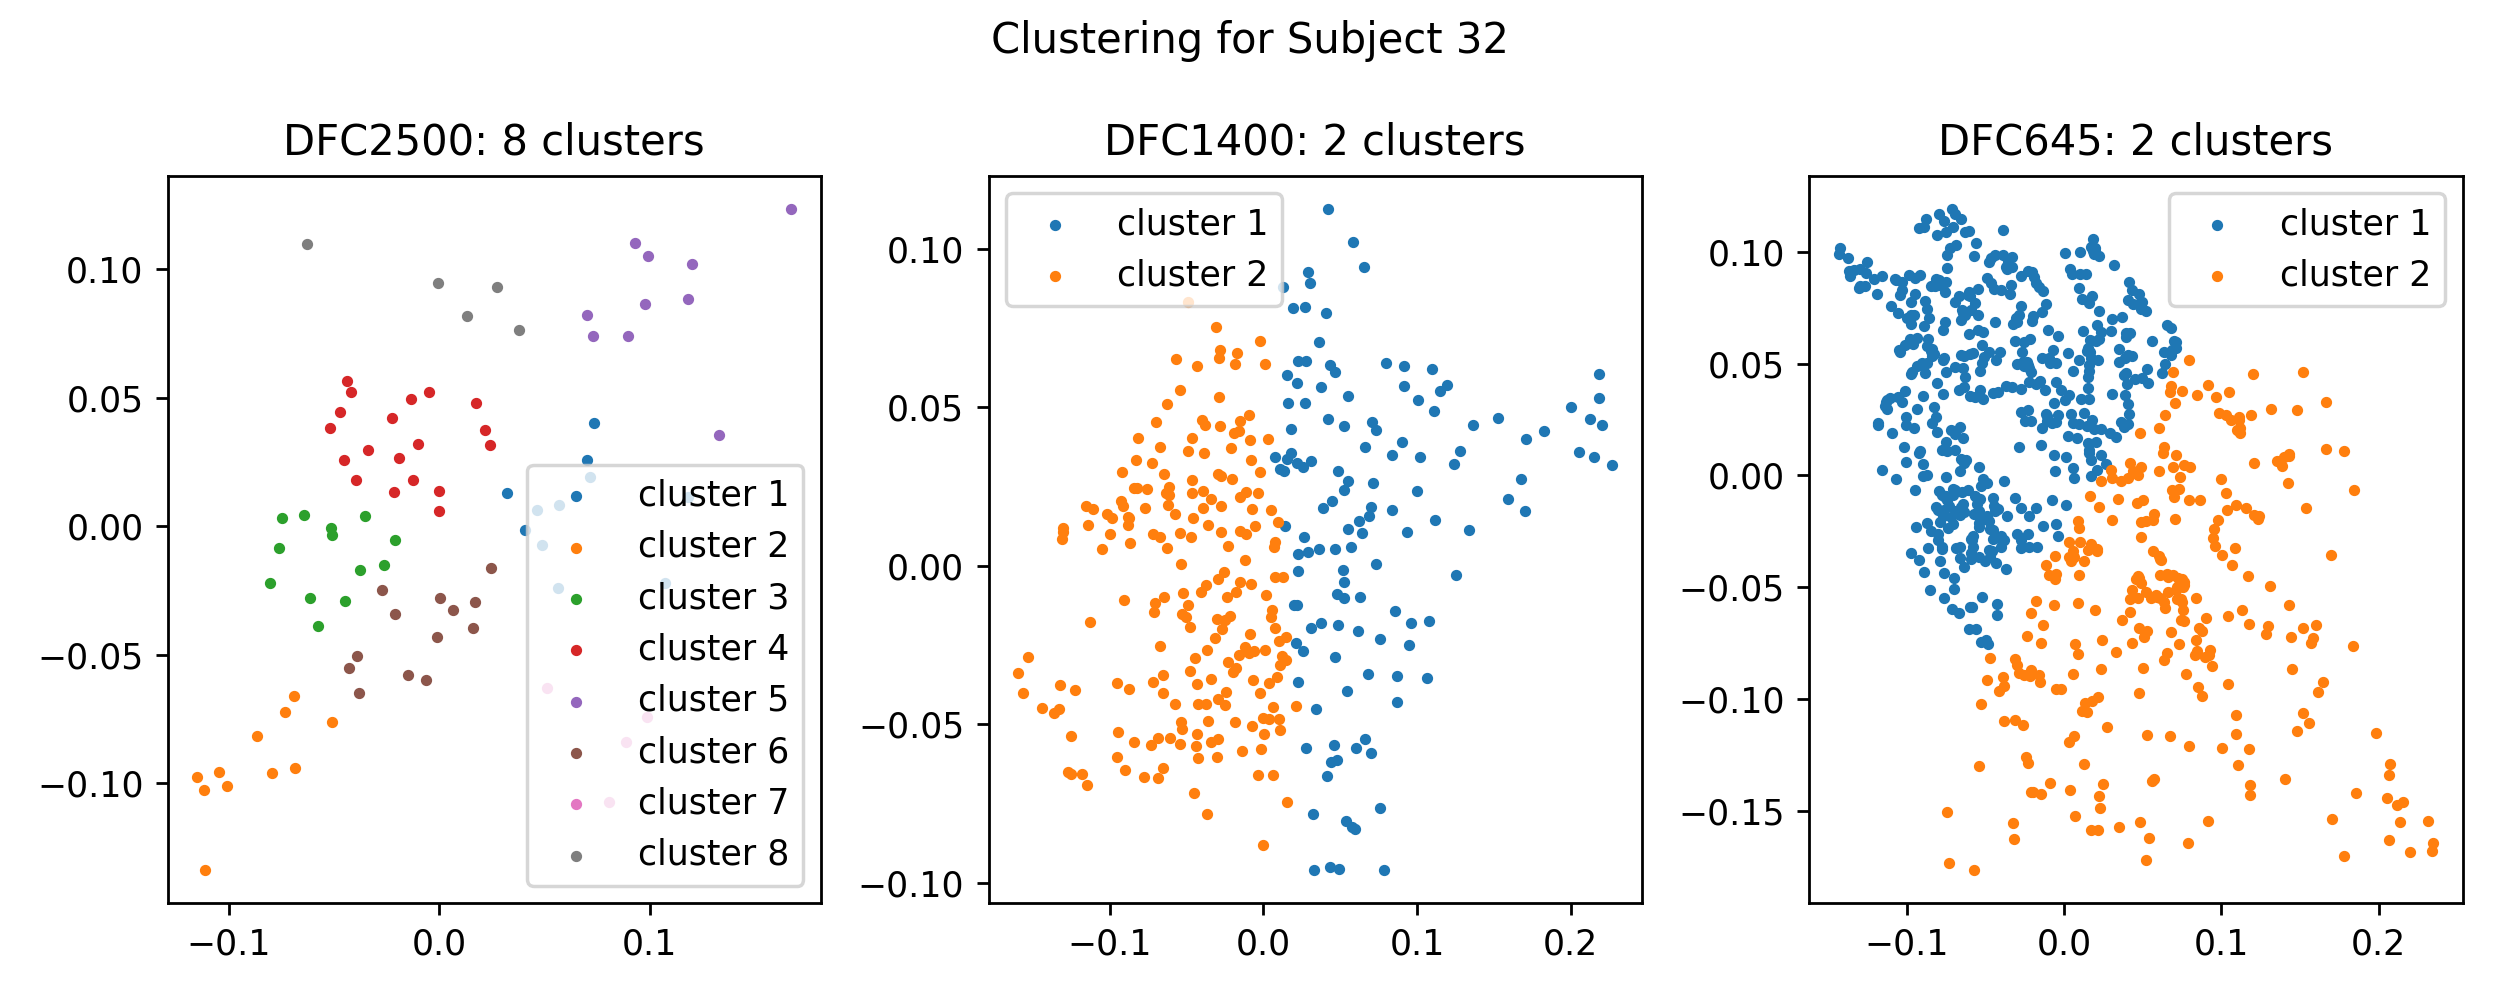
\includegraphics[width=1\textwidth, trim={0cm, 0.0cm, 0.0cm, 0.0cm}]{figures/new_formula_tda_bn_subject_32.png}\hfill
		%\hspace{-15mm}
	\end{subfigure}
	\begin{subfigure}[t]{1\textwidth}
		\centering
		\hspace{8mm}
		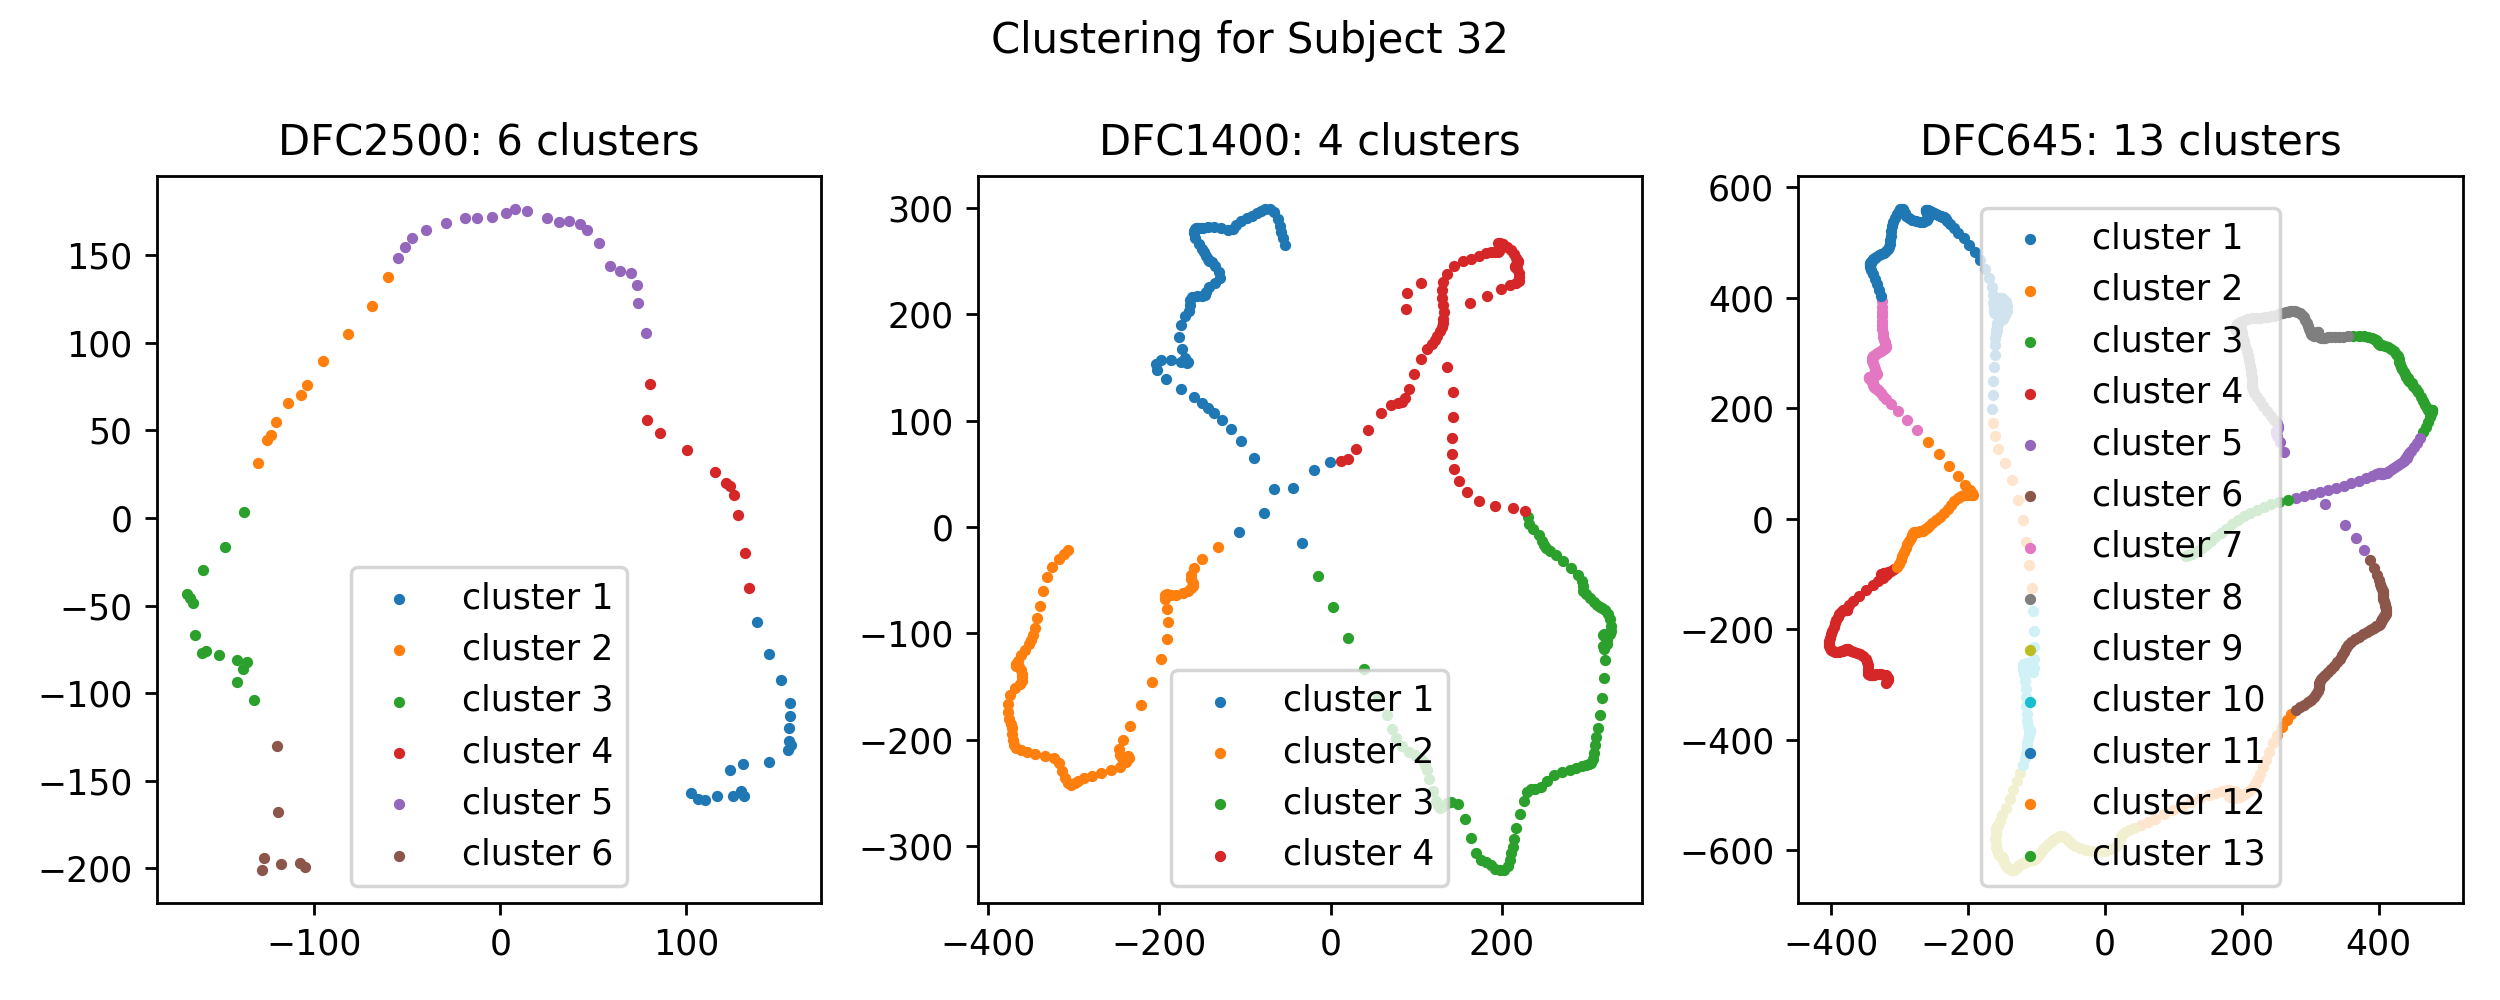
\includegraphics[width=1\textwidth, trim={0cm, 0.0cm, 0.0cm, 0.0cm}]{figures/new_formula_nontda_subject_32.png}\hfill
		%\hspace{-15mm}
	\end{subfigure}
	\caption{Clustering result for subject $32$ (top row) for temporal period $2500ms$ (left), $1400ms$ (center), and $645ms$ (right) using $1 - corr$ formula and Bottleneck distance. Clustering result for the same subject (bottom row) with NonTDA Clustering result.}
	\label{fig:clus_new_formula}
\end{figure}

Figure \ref{fig:clus_new_formula} shows the clustering result for a single subject (subject 32) for all three data cohorts ($2500ms$, $1400ms$, $645ms$). The top row of the figure represents the plotted clusters using the TDA pipeline using Bottleneck distance. The bottom row of the figure shows the plotted clusters for the same subject using the nonTDA pipeline, and the number of clusters varies for the data cohorts. 

\setlength{\tabcolsep}{0.5em} % for the horizontal padding
{\renewcommand{\arraystretch}{1.2}% for the vertical padding
    \begin{table}[t]
        \centering
        \begin{tabular}
        {| c | c | c | c | c |}
         \hline
            \multirow{2}{*}{Distance} & \multicolumn{2}{c |}{TDA Pipeline} & \multicolumn{2}{c |}{NonTDA Pipeline} \\ \cline{2-5}
              & Subjects & Percentage & Subjects & Percentage
             \\ \hline \hline
             0 & 109 & 34.49\% & 4 & 1.27\% \\ \hline 
             1 & 50 & 15.82\% & 5 & 1.58\% \\ \hline 
             2 & 39 & 12.34\% & 11 & 3.48\% \\ \hline 
             3 & 26 & 8.23\% & 18 & 5.70\% \\ \hline 
             4 & 27 & 8.54\% & 22 & 6.96\% \\ \hline 
             5 & 11 & 3.48\% & 30 & 9.49\% \\ \hline 
             6 & 11 & 3.48\% & 20 & 6.33\% \\ \hline 
             7 & 5 & 1.58\% & 23 & 7.28\% \\ \hline 
             8 & 6 & 1.90\% & 39 & 12.34\% \\ \hline 
             9 & 5 & 1.58\% & 34 & 10.76\% \\ \hline 
             10 & 5 & 1.58\% & 36 & 11.39\% \\ \hline 
             11 & 6 & 1.90\% & 43 & 13.61\% \\ \hline 
             12 & 8 & 2.53\% & 21 & 6.65\% \\ \hline 
             13 & 8 & 2.53\% & 10 & 3.16\% \\ \hline 
             
        \end{tabular}
        \caption{Distance between the number of clusters for the data cohorts for TDA (BN) and NonTDA pipeline using Eq. \ref{eq:dis}}
         \label{tab:clustering_new_formula}
    \end{table}   

We capture the number of clusters for 316 subjects for all three data cohorts for both pipelines with this mapping using Equaltion \ref{eq:dis}. Table \ref{tab:clustering_new_formula} shows the distance analysis for both of the pipelines. In the TDA pipeline with Bottleneck distance, we see that majority of the subjects ($59\%$) have a distance less than or equal to one for the data cohorts. On the other hand, in the nonTDA pipeline, less than $3\%$ of the subjects have a distance less than or equal to one. We also perform a pairwise comparison of the number of clusters for the data cohorts for both of the pipelines. Table \ref{tab:tda_between_new_ws} shows the pairwise distance between the data cohorts in the TDA pipeline using Wasserstein distance. Table \ref{tab:tda_between_new_bn} shows the pairwise distance between the data cohorts in the TDA pipeline using Bottleneck distance. Table \ref{tab:nontda_between_new_eu} shows the pairwise distance between the data cohorts in the traditional FCN analysis pipeline (nonTDA). 

    \begin{table}[t]
        \centering
        \begin{tabular}
        {| c | c | c | c | c | c | c |}
         \hline
            \multirow{2}{*}{Distance} & \multicolumn{2}{c |}{$2500ms$ and $1400ms$ } & \multicolumn{2}{c |}{$1400ms$ and $645ms$ } & \multicolumn{2}{c |}{$645ms$ and $2500ms$ } \\ \cline{2-7}
              & Subjects & Percentage & Subjects & Percentage & Subjects & Percentage
             \\ \hline \hline
0 & 120 & 37.975\% & 100 & 31.646\% & 123 & 38.924\% \\ \hline 
1 & 51 & 16.139\% & 49 & 15.506\% & 44 & 13.924\% \\ \hline 
2 & 24 & 7.595\% & 32 & 10.127\% & 19 & 6.013\% \\ \hline 
3 & 19 & 6.013\% & 18 & 5.696\% & 21 & 6.646\% \\ \hline 
4 & 15 & 4.747\% & 15 & 4.747\% & 15 & 4.747\% \\ \hline 
5 & 14 & 4.430\% & 12 & 3.797\% & 15 & 4.747\% \\ \hline 
6 & 13 & 4.114\% & 10 & 3.165\% & 13 & 4.114\% \\ \hline 
7 & 13 & 4.114\% & 19 & 6.013\% & 12 & 3.797\% \\ \hline 
8 & 4 & 1.266\% & 8 & 2.532\% & 5 & 1.582\% \\ \hline 
9 & 7 & 2.215\% & 9 & 2.848\% & 10 & 3.165\% \\ \hline 
10 & 10 & 3.165\% & 10 & 3.165\% & 14 & 4.430\% \\ \hline 
11 & 11 & 3.481\% & 7 & 2.215\% & 4 & 1.266\% \\ \hline 
12 & 6 & 1.899\% & 8 & 2.532\% & 8 & 2.532\% \\ \hline 
13 & 9 & 2.848\% & 19 & 6.013\% & 13 & 4.114\% \\ \hline 
        \end{tabular}
        \caption{Clustering result similarity between cohorts for TDA pipeline using 1 - correlation formula and WS distance}
        \label{tab:tda_between_new_ws}
    \end{table}    
    

    \begin{table}[t]
        \centering
        \begin{tabular}
        {| c | c | c | c | c | c | c |}
         \hline
            \multirow{2}{*}{Distance} & \multicolumn{2}{c |}{$2500ms$ and $1400ms$ } & \multicolumn{2}{c |}{$1400ms$ and $645ms$ } & \multicolumn{2}{c |}{$645ms$ and $2500ms$ } \\ \cline{2-7}
              & Subjects & Percentage & Subjects & Percentage & Subjects & Percentage
             \\ \hline \hline
0 & 143 & 45.253\% & 189 & 59.810\% & 141 & 44.620\% \\ \hline 
1 & 52 & 16.456\% & 41 & 12.975\% & 45 & 14.241\% \\ \hline 
2 & 44 & 13.924\% & 28 & 8.861\% & 37 & 11.709\% \\ \hline 
3 & 19 & 6.013\% & 16 & 5.063\% & 21 & 6.646\% \\ \hline 
4 & 21 & 6.646\% & 8 & 2.532\% & 23 & 7.278\% \\ \hline 
5 & 5 & 1.582\% & 8 & 2.532\% & 10 & 3.165\% \\ \hline 
6 & 5 & 1.582\% & 7 & 2.215\% & 6 & 1.899\% \\ \hline 
7 & 4 & 1.266\% & 1 & 0.316\% & 4 & 1.266\% \\ \hline 
8 & 6 & 1.899\% & 3 & 0.949\% & 4 & 1.266\% \\ \hline 
9 & 3 & 0.949\% & 6 & 1.899\% & 7 & 2.215\% \\ \hline 
10 & 1 & 0.316\% & 2 & 0.633\% & 4 & 1.266\% \\ \hline 
11 & 5 & 1.582\% & 5 & 1.582\% & 5 & 1.582\% \\ \hline 
12 & 3 & 0.949\% & 2 & 0.633\% & 4 & 1.266\% \\ \hline 
13 & 5 & 1.582\% & 0 & 0.000\% & 5 & 1.582\% \\ \hline 
        \end{tabular}
        \caption{Clustering result similarity between cohorts for TDA pipeline using 1 - correlation formula and BN distance}
        \label{tab:tda_between_new_bn}
    \end{table}    


    \begin{table}[t]
        \centering
        \begin{tabular}
        {| c | c | c | c | c | c | c |}
         \hline
            \multirow{2}{*}{Distance} & \multicolumn{2}{c |}{$2500ms$ and $1400ms$ } & \multicolumn{2}{c |}{$1400ms$ and $645ms$ } & \multicolumn{2}{c |}{$645ms$ and $2500ms$ } \\ \cline{2-7}
              & Subjects & Percentage & Subjects & Percentage & Subjects & Percentage
             \\ \hline \hline
0 & 21 & 6.646\% & 37 & 11.709\% & 12 & 3.797\% \\ \hline 
1 & 29 & 9.177\% & 36 & 11.392\% & 21 & 6.646\% \\ \hline 
2 & 43 & 13.608\% & 40 & 12.658\% & 27 & 8.544\% \\ \hline 
3 & 28 & 8.861\% & 39 & 12.342\% & 29 & 9.177\% \\ \hline 
4 & 38 & 12.025\% & 39 & 12.342\% & 34 & 10.759\% \\ \hline 
5 & 30 & 9.494\% & 29 & 9.177\% & 30 & 9.494\% \\ \hline 
6 & 23 & 7.278\% & 22 & 6.962\% & 14 & 4.430\% \\ \hline 
7 & 18 & 5.696\% & 20 & 6.329\% & 22 & 6.962\% \\ \hline 
8 & 20 & 6.329\% & 22 & 6.962\% & 26 & 8.228\% \\ \hline 
9 & 18 & 5.696\% & 17 & 5.380\% & 25 & 7.911\% \\ \hline 
10 & 16 & 5.063\% & 9 & 2.848\% & 23 & 7.278\% \\ \hline 
11 & 22 & 6.962\% & 3 & 0.949\% & 33 & 10.443\% \\ \hline 
12 & 6 & 1.899\% & 1 & 0.316\% & 15 & 4.747\% \\ \hline 
13 & 4 & 1.266\% & 2 & 0.633\% & 5 & 1.582\% \\ \hline 
        \end{tabular}
        \caption{Clustering result similarity between cohorts for NON TDA pipeline using 1 - correlation formula and EU distance}
        \label{tab:nontda_between_new_eu}
    \end{table}        
      


